% A cantilever modelled with six nodes but only one joint (node 1)
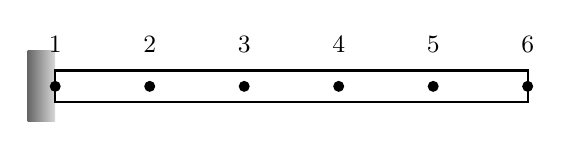
\begin{tikzpicture}[scale=1.0,font=\small]
  \fill[left color=black!60,right color=black!15] (-0.35,-0.45) rectangle (0,0.45);
  \draw[thick] (0,-0.2) rectangle (6,0.2);
  \foreach \i in {1,...,6}{
    \fill ({(\i-1)*1.2},0) circle (0.07);
    \node[above] at ({(\i-1)*1.2},0.3) {\i};}
\end{tikzpicture}
